\documentclass[crop,tikz]{standalone}% 'crop' is the default for v1.0, before it was 'preview'
\usetikzlibrary{shapes.geometric, shapes, hobby}

\begin{document}

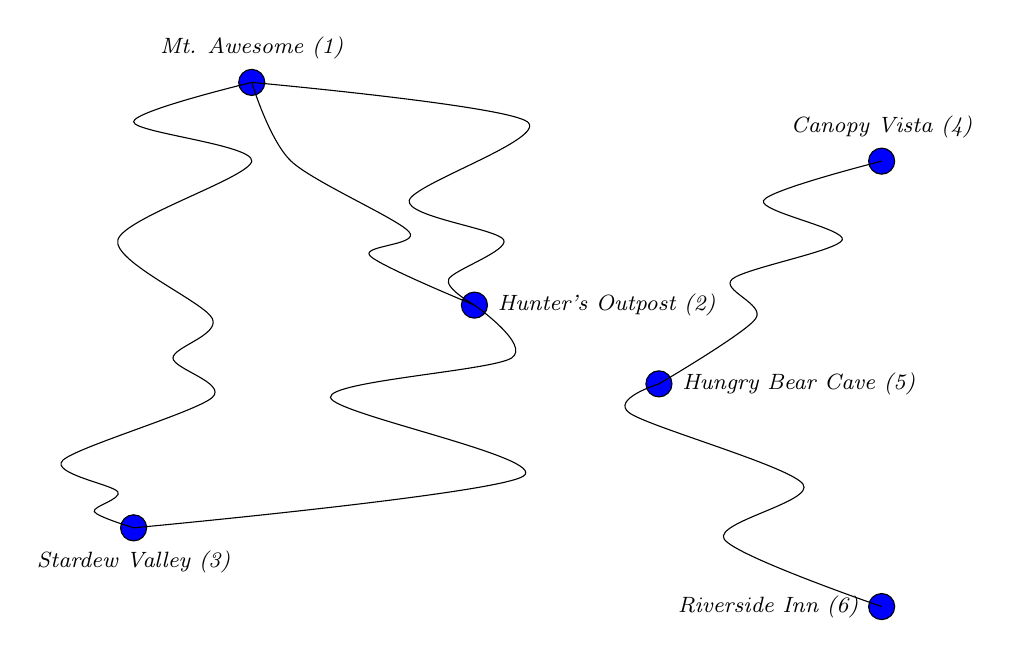
\begin{tikzpicture}
\tikzset{
node distance=4 cm,
dot/.style={draw,shape=circle,fill=blue},
every label/.style = {font=\footnotesize\itshape},
smooth
}

	% coordinates
	% \draw[help lines] (0,0) grid (15,15);

	\node[dot, label=above:Mt. Awesome (1)] at (2, 10) (1) {};
	\node[dot, below right of=1, label=right:Hunter's Outpost (2)] (2) {};
	\node[dot, below left of=2,label=below:Stardew Valley (3), xshift=-1.5cm] (3) {};


	\node[dot, label=above:Canopy Vista (4)] at (10,9) (4) {};
	\node[dot, below left of=4, label=right:Hungry Bear Cave (5)] (5) {};
	\node[dot, below right of=5, label=left:Riverside Inn (6)]  (6) {};

	\draw plot coordinates {(1) (0.5,9.5) (2,9) (0.3,8) (1.5,7) (1,6.5) (1.5,6) (-0.4,5.2) (0.3,4.8) (0,4.55) (3)};

	\draw plot coordinates {(1) (5.5,9.5) (4,8.5) (5.2,8) (4.5,7.5) (2)};
	\draw plot coordinates {(1) (2.5,9) (4,8.1) (3.5, 7.8) (2)};
	\draw plot coordinates {(2) (5.3,6.5) (3,6) (5.45, 5) (3)};

	\draw plot coordinates {(4) (8.5,8.5) (9.5,8) (8.1,7.5) (8.4,7) (5)};
	\draw plot coordinates {(5) (6.8,5.8) (9,4.9) (8,4.2) (6)};

\end{tikzpicture}
\end{document}
